\section{Windows}

Officially, the pbdR team does not support gaming consoles (only kidding!).  Jokes aside, it is possible to install a pbdR environment on Windows, but it is not necessarily the easiest.  This guide will explain the basics of getting \proglang{R}, OpenMPI, and pbdR installed on your Windows system.  The instructions and screenshots for this document are for version 2.15.1 of R, but later versions should be very similar, if not identical.

If you are completely new to \proglang{R}, then you may find the \href{http://cran.r-project.org/bin/windows/base/rw-FAQ.html}{R for Windows FAQ} useful.  Additionally, there is also an \href{http://cran.r-project.org/doc/FAQ/R-FAQ.html}{R FAQ} which may also be useful for those who know very little about \proglang{R}.  To learn more about programming with \proglang{R}, then you may find the \href{http://cran.us.r-project.org/doc/manuals/R-intro.html}{Introduction to R} guide useful.


\subsection{Installing R}


\begin{enumerate}
  \item Download R: \url{http://cran.r-project.org/bin/windows/base/} \label{enum:windl}
  \sshots{\begin{center}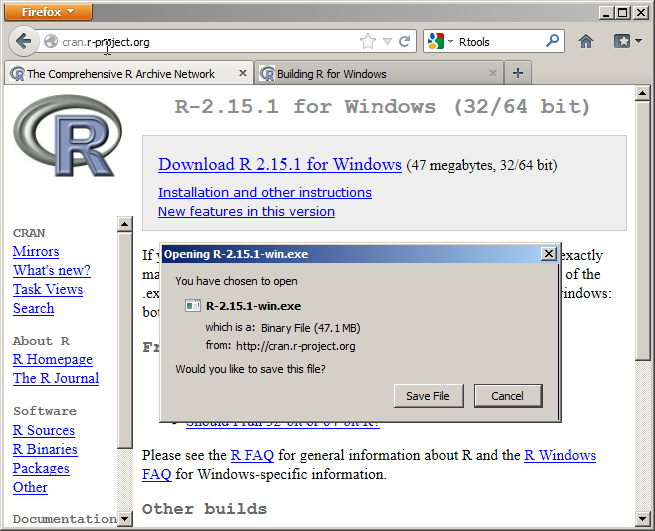
\includegraphics[scale=.5]{windows/pics/R_1.png}\end{center}}
  %
  \item Open the saved file from \ref{enum:windl} above to begin the installation.  At the first setup screen, click 'Next' to continue.
  \sshot{windows/pics/R_2.png}
  %
  \item When prompted with the license, click 'Next' to continue.
  \sshot{windows/pics/R_3.png}
  %
  \item When prompted for the location to install R, we strongly encourage you to use the default.  When you have made your decision, click 'Next'.
  \sshot{windows/pics/R_4.png}
    %
  \item When prompted with the components to install, you should select a 'User installation'.  Then click 'Next'.
  \sshot{windows/pics/R_5.png}
    %
  \item When prompted with the option to alter the startup options, we suggest selecting \code{No (accept defaults)}.  When you have made your decision, click 'Next'.
  \sshot{windows/pics/R_6.png}
    %
  \item When prompted with the start menu folder options, make your choice and then click 'Next'.
  \sshot{windows/pics/R_7.png}
    %
  \item When prompted with the additional tasks options, we suggest making sure that \code{Save version number in registry} and \code{Associate R with .RData files} are both \textbf{checked}.  When you have made your decisions, click 'Next'.
  \sshot{windows/pics/R_8.png}
  %
  \item To complete the R installation, select 'Finish'.
  \sshot{windows/pics/R_9.png}
  %
\end{enumerate}

Once \proglang{R} is finished installing, you need to install the  \href{http://cran.r-project.org/web/packages/rlecuyer/index.html}{\pkg{rlecuyer}} package.  To install it from an interactive \proglang{R} session, simply start an \proglang{R} session and issue the command
\begin{lstlisting}[language=rr]
install.packages("rlecuyer")
\end{lstlisting}





\subsection{Installing Rtools}\label{inst:rtools}

\begin{enumerate}
  \item Download Rtools: \url{http://cran.r-project.org/bin/windows/base/} \label{enum:rtoolsdl}
  \sshots{\begin{center}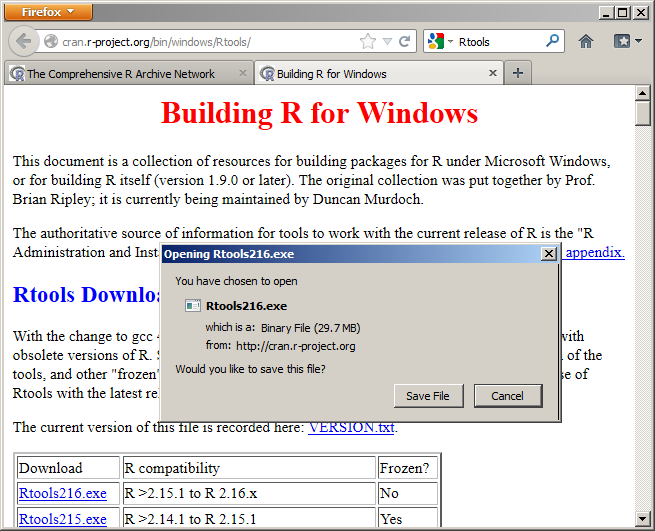
\includegraphics[scale=.5]{windows/pics/Rtools_1.png}\end{center}}
  %
  \item Open the saved file from \ref{enum:rtoolsdl} above to begin the installation.  At the first setup screen, click 'Next' to continue.
  \sshot{windows/pics/Rtools_2.png}
  %
  \item When prompted with the license, click 'Next' to continue.
  \sshot{windows/pics/Rtools_3.png}
  %
  \item When prompted for the location to install R, we strongly encourage you to use the default.  When you have made your decision, click 'Next'.
  \sshot{windows/pics/Rtools_4.png}
    %
  \item When prompted with the components to install, you should select a 'User installation'.  Then click 'Next'.
  \sshot{windows/pics/Rtools_5.png}
    %
  \item When prompted with the option to alter the startup options, we suggest selecting \code{No (accept defaults)}.  When you have made your decision, click 'Next'.
  \sshot{windows/pics/Rtools_6.png}
    %
  \item When prompted with the start menu folder options, make your choice and then click 'Next'.
  \sshot{windows/pics/Rtools_7.png}
    %
  \item To complete the Rtools installation, select 'Finish'.
  \sshot{windows/pics/Rtools_8.png}
  %
\end{enumerate}





\subsection{Installing MPI}
Before proceeding, please be aware that this installation requires {\color{red}{administrative privileges}}.

\begin{enumerate}
  \item Download both the 32-bit
  \href{http://www.mpich.org/static/tarballs/1.4.1p1/mpich2-1.4.1p1-win-ia32.msi}{mpich2-1.4.1p1-win-i32.msi} 
  and the 64-bit
  \href{http://www.mpich.org/static/tarballs/1.4.1p1/mpich2-1.4.1p1-win-x86-64.msi}{mpich2-1.4.1p1-win-x86-64.msi}
  installers from: \url{http://www.mpich.org/} .\label{enum:mpich2}
  \sshots{\begin{center}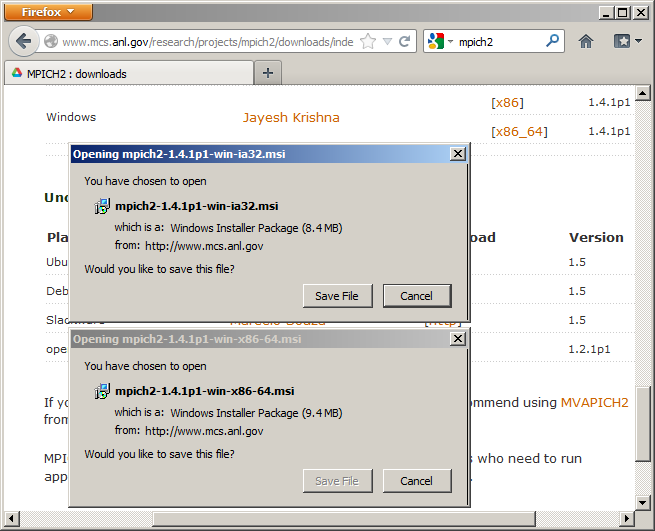
\includegraphics[scale=.5]{windows/pics/mpich2_1.png}\end{center}}
  %
  \item Open the saved file from \ref{enum:mpich2} above to begin the installation.  At the first setup screen, click 'Next' to continue.
  \sshot{windows/pics/mpich2_2.png}
  %
  \item When prompted with the system requirements, click 'Next' to continue.
  \sshot{windows/pics/mpich2_3.png}
  %
  \item When prompted with the license, click ``I agree'' and then click 'Next' to continue.
  \sshot{windows/pics/mpich2_4.png}
    %
  \item When prompted with the 'Process Manager setup' screen, choose a passphrase and then click 'Next' to continue.
  \sshot{windows/pics/mpich2_5.png}
    %
  \item At the 'Select Installation Folder' screen, we recommend you keep the default folders.  By default, the 32-bit application will be installed in \code{C:\textbackslash Program Files (x86)\textbackslash MPICH2\textbackslash } and the 64bit application will be installed in \code{C:\textbackslash Program Files\textbackslash MPICH2\textbackslash }.\\[.2cm] Additionally, you should make the selection for whether or not MPICH2 should be available to all users of this system or just yourself.  When you are ready to proceed, click 'Next'.
  \sshot{windows/pics/mpich2_6.png}
  \sshot{windows/pics/mpich2_6_1.png}
    %
  \item When prompted to confirm the installation, click 'Next' to proceed.
  \sshot{windows/pics/mpich2_7.png}
    %
  \item To complete the MPICH2 installation, select 'Close'.
  \sshot{windows/pics/mpich2_8.png}
  %
\end{enumerate}






\subsection{Installing pbdR Packages}

Unfortunately, we do not distribute pbdR binary packages on the CRAN for Windows.  This means that you must install our packages from source on Windows, and the process may be foreign.  We will present two approaches; the short way, installing from github using the \pkg{devtools} package, and a longer way, installing from a downloaded source file.  However, do be aware that each of these methods requires the installation of the Rtools package from Section~\ref{inst:rtools} (so that step cannot be skipped).

Finally, we note that it may not be possible to install the \pkg{pbdNCDF4} package on Windows.  We have not tested this and, assuming it is possible, it would be very difficult to get NetCDF4 compiled in parallel first.  If you have success installing this package on Windows, we would love to hear from you.


\subsubsection{Installing from Github}

This is probably the simplest method, assuming that you have Rtools installed and set up correctly.  If Rtools is not in your PATH, then you may need to enter something like the following:
\begin{lstlisting}[language=rr]
rtools <- "C:\\Rtools\\bin\\"
mingw <- "C:\\Rtools\\gcc-4.6.3\\bin\\"

PATH <- Sys.getenv("PATH")
new.PATH <- paste(rtools, mingw, PATH, sep = ";")
Sys.setenv(PATH=new.PATH)
\end{lstlisting}
Where the \code{rtools} and \code{mingw} directories are as they are on your machine.

Once that is settled, installing is fairly simple.  You simply load the \pkg{devtools} package and install from our github repo as follows:
\begin{lstlisting}[language=rr]
library(devtools)

install_github(repo="pbdMPI", username="RBigData")
install_github(repo="pbdSLAP", username="RBigData")
install_github(repo="pbdBASE", username="RBigData")
install_github(repo="pbdDMAT", username="RBigData")
install_github(repo="pbdDEMO", username="RBigData")
\end{lstlisting}

You can also install \emph{really} new package builds, which will be very current in terms of features, but also bugs (or even complete package breakage).  If you're sure you want these packages, then you can install them as follows:

\begin{lstlisting}[language=rr]
# dev repo 1
install_github(repo="pbdMPI", username="snoweye")
install_github(repo="pbdSLAP", username="snoweye")
# dev repo 2
install_github(repo="SEXPtools", username="wrathematics")
install_github(repo="pbdBASE", username="wrathematics")
install_github(repo="pbdDMAT", username="wrathematics")
install_github(repo="pbdDEMO", username="wrathematics")
\end{lstlisting}



\subsubsection{Installing from Downloaded Source}

\begin{enumerate}
  \item To help simplify things, we offer a simple \href{https://github.com/wrathematics/installation-instructions/raw/master/windows/build_pbdMPI.bat}{install script} which makes managing the \code{PATH} slightly simpler.  By default, this is for \proglang{R} version 2.15.3 and \pkg{pbdMPI} version 0.1-6.  If you have a different version of R or want to install a different version of \pkg{pbdMPI}, simply change lines 4 and/or 5 of the install script to match your needs.
  \sshot{windows/pics/build_0.png}
  %
  \item Open a command prompt either from the start menu, or by entering the command \code{Windows key} then \code{R}, and then entering \code{cmd} in the ``run'' dialog box.
  \sshot{windows/pics/build_1.png}
  %
  \item Before proceeding further, it is probably a good idea to test the installation of MPICH2.  The following commands utilize MPICH2 to do some fairly trivial things (do not copy \code{SHELL>} if you are copying and pasting from the lines below):
\begin{lstlisting}[language=sh]
SHELL> C:\PROGRA~1\MPICH2\bin\mpiexec -np 2 hostname.exe
SHELL> C:\PROGRA~1\R\R-2.15.1\bin\R --vanilla --slave -e "ls()"
SHELL> C:\PROGRA~1\R\R-2.15.1\bin\Rscript --vanilla --slave -e "ls()"
\end{lstlisting}
  \sshot{windows/pics/build_2.png}
  %
%   \item Next, go download and install the \href{http://cran.r-project.org/web/packages/rlecuyer/index.html}{\pkg{rlecuyer}} package.
%   \sshot{windows/pics/build_3.png}
  %
  \item Download the \href{http://cran.r-project.org/src/contrib/pbdMPI_0.1-6.tar.gz}{source} for \href{http://cran.r-project.org/web/packages/pbdMPI/index.html}{\pkg{pbdMPI}} package.  Put it in the same directory as your \code{build_pbdMPI.bat} file, and then execute \code{build_pbdMPI.bat} from the command prompt to install the package.
  \sshot{windows/pics/build_4.png}
    %
  \item If the process is done without errors, you can see the binary package is installed. 
  \sshot{windows/pics/build_5.png}
%     %
%   \item 
%   \sshot{windows/pics/build_6.png}
\end{enumerate}
